\chapter{Introduction}
\label{chap:Intro}

\epigraph{It is hard for me to say confidently that, after fifty more 
years of explosive growth of computer science, there will still be a 
lot of fascinating unsolved problems at peoples' fingertips, that it 
won't be pretty much working on refinements of well-explored things. 
Maybe all of the simple stuff and the really great stuff has been 
discovered. It may not be true, but I can't predict an unending growth. 
I can't be as confident about computer science as I can about biology. 
Biology easily has 500 years of exciting problems to work on, it's at 
that level.}{\textit{--- Donald Knuth}}

\section{About this document} 

These document contains the content of modules on Biological Computing 
taught in various courses at the Department of Life Sciences, Imperial 
College London. These courses include Year 1\&2 Computational 
Biostatistics modules at the South Kensington Campus, the MSc/MRes 
on Computational Methods in Ecology and Evolution (CMEE Masters) at Silwood 
Park, and the Quantitative Methods in Ecology and Evolution Centre for 
Doctoral Training (QMEE CDT).

Different subsets of this document will be covered in different 
courses. Please look up your respective course guidebooks/handbooks to determine when the 
modules covered in these notes are scheduled in your course. 
You will be given instructions about which sections are covered in your 
course. 

This document is accompanied by data and code on which you can practice 
your skills in your own time and during the practical sessions. These 
materials are available (and will be updated regularly) at: 
\url{https://bitbucket.org/mhasoba/silbiocompmasterepo}. 
I use git for hosting this course's materials because I want to 
version-control this course's content, which is constantly evolving to 
keep up with changing programming/computing technologies. That is, I am treating 
this course as any computing 
project that needs to be regularly updated and improved. Changes to the 
notes and content will also be made based upon students' feedback. 
Blackboard is just not set up to handle dynamic updating and version 
control of this sort! You will see tips like this in the following 
chapters that you should pay special attention to:
\begin{tipbox}
If you do not use git (or are not required to do so!), you may download 
the code, data, these notes, and other course materials from the 
bitbucket repository at one go, by going to 
\url{https://bitbucket.org/mhasoba/silbiocompmasterepo/downloads} and 
then clicking on the ``Download repository'' link. You can then unzip 
the downloaded .zip and grab the files you need. 
\end{tipbox}

\begin{wrapfigure}[13]{c}{0.5\textwidth}
   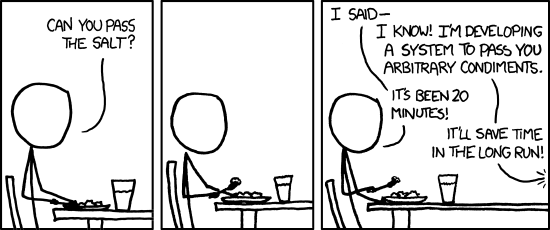
\includegraphics[width=1\linewidth]{programming.png}
	\caption{\label{fig:Programming} But not every task needs to be 
	converted to a computer program --- you will learn to decide when to 
	and when not to write a computer program! \url{http://xkcd.com/974/}} 
\end{wrapfigure}
It is important that you work through the exercises and problems in 
each chapter/section. This document does not tell you every single 
thing you need to know to perform the exercises in it. In programming 
and computing, you learn faster by trying to solve problems (including 
computer crashes!) on your own, often by liberally googling the problem! 

You will be provided guidelines for what makes good or efficient 
solutions to the computing exercises. Later, when you have submitted 
your exercises and practicals, you will be provided solutions. 

Also, every time a mysterious, geeky-sounding term like ``relative 
path'' or ``version control'' appears, please google it!

\section{The goals of this course}

The goal of this course is to teach you to become (or at least show you 
the path towards becoming) a competent quantitative biologist. A large 
part of this involves learning computer programming. Why do biologists 
need to write write computer programs? Here are some (hopefully 
compelling to you!) reasons:

\begin{itemize} \itemsep0pt
	\item Short of fieldwork, programs can do anything (that can be 
	specified). In fact, even fieldwork, if you could one day {\it 
	program} a robot to do it for you \footnote{That way you can potter around
	the forest catching rare butterflies and frogs while the robot does the boring 
	data collecting for you}!  

	\item As such, no software is typically available to perform exactly 
	the analysis you are planning. You should be unhappy if you are 
	trying to shoehorn your data into methods that don't quite seem 
	right.
	
	\item Biological problems and datasets are some of the most 
	complicated imaginable. Programming permits success despite 
	complexity through precise specification	and modularization of 
	complicated analyses. 
	
	\item Modularity -- programming allows you to break up your complex 
	analysis in smaller pieces, yet keep all the pieces in a single, 
	functional analysis.
	 
	\item Reproducibility -- you (or someone else) can just re-run the 
	code to reproduce your analysis. This is also the key to maintaining 
	scientific accountability, integrity, and accuracy.

	\item Organised thinking -- writing code requires you to do this!
	
	\item Career prospects -- good, scientific coders are in short supply 
	in all fields, but most definitely in biology!
	
\end{itemize}

There are several hundred programming languages currently available -- 
which ones should a biologist choose? Ideally, a quantitative biologist 
would like to know:
\begin{enumerate}
	\item A {\it fast}, compiled (or semi-compiled) `procedural' language 
	like {\tt C}
	\item A modern, easy-to-write, interpreted (or semi-compiled) 
	language that is still quite fast, like {\tt python}
	\item A mathematical/statistical software with programming and 
	graphing capabilities like {\tt R}
\end{enumerate}
And all these because one language doesn't fit all purposes. Therefore you 
will learn a few different languages in this course --- hopefully, just 
the right number! Among the languages you will learn here --- {\tt 
python}, 
{\tt R}, and {\tt C} are three of the most popular currently (see
\url{https://www.tiobe.com/tiobe-index/} and \url{ https://goo.gl/vyrqr1}, 
and for some very good reasons.

Our goal is to teach you not just programming, but also good computing 
practices. In this course, you will write plenty of code, deal with 
different data files, and produce text and graphic outputs. You will 
learn to keep your project and coursework organized in logical, 
efficient, error-free and reproducible {\it workflows} (that's a 
mouthful, but an important mouthful).

\section{Some guidelines, conventions and rules} 

\subsection{Beware the dark forces} 

You will NOT be using spreadsheet software (e.g., Excel) in these classes. 
There are times when you will feel the pull of the dark side (ahem!), 
and imagine a more ``comfortable'' world where you are 
mouse-clicking your way happily though Excel-based data manipulations 
and analyses. NO! You will be doing yourself a disservice. On the 
long-ish run you will be much better off visualizing and manipulating 
data on your computer using a programming language like R. This is something you will learn, young {\it padawan}!  

\subsection{Keep your workflow organized}
In the following chapters, you will practice many examples where you 
are required to write large blocks of code. Please get into the habit 
of writing code into text files with an appropriate extension (e.g., 
{\tt *.R} for {\tt R} code, {\tt *.py} for {\tt python} code, etc.). 
Furthermore, please keep all your code files organized in one or more 
directories (e.g., named {\tt Code}!). Similarly, some of these scripts 
will take data files as inputs, and output some results in the form of 
text or graphics. Please keep these inputs and outputs organized as 
well, in separate directories (e.g., named {\tt Data} and {\tt 
Results}) respectively. Your demonstrators and I will help you get set 
up and abide by this ``workflow''. 

\subsection{Conventions used in this document}

Throughout this document, directory paths will be specified in UNIX 
(Mac, Linux) style, using $/$ instead of the \textbackslash{} used in 
Windows. Also, in general, we will be using {\it relative paths} 
throughout the exercises and practicals (more on this later, but google 
it!).

You will find all command line/console arguments, code snippets and 
output in coloured boxes like this:
\begin{lstlisting}
$ ls 
$
\end{lstlisting}
The specific prompt (\$ in this case, belonging to the UNIX terminal) 
will vary with the programming language/console ({\tt \$} for UNIX, 
$>>>$ for Python, {\tt >} for R, etc.).

You will type the commands/code that you see in such boxes 
into the relevant command line (or copy-paste, but not recommended!). I 
have aimed to make the content of this module computer platform (Mac, 
Linux or PC) independent. Also note that:\\

\begin{compactitem}[$\quad\star$]\itemsep4pt
	\item Lines marked with a star like this will be specific 
	instructions for you to follow
\end{compactitem}

\begin{wrapfigure}[20]{c}{0.4\textwidth}
 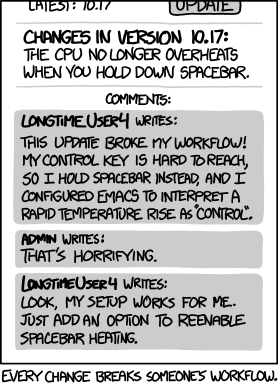
\includegraphics[width=1\linewidth]{workflow.png}
	\caption{\label{fig:Workflows} Logical workflows are important, but 
	don't get married to yours! \url{http://xkcd.com/1172/} } 
\end{wrapfigure}

\subsection{To IDE or not to IDE?}

As you embark on your journey to becoming a competent prectioner of 
biological computing, you will be faced with a hamletian question: ``To 
IDE or not to IDE''. OK, maybe not that dramatic or hamletian... 

An interactive Development Environment (IDE) is a text editor with 
frills that can make life easy by auto-formatting code, running code 
though the terminal or command line, allowing a graphic view of the 
workspace (your active functions, variables, etc.), graphic debugging 
and profiling (you will see these delightful things later), and 
allowing integrated version control (e.g., using {\tt git}). You will 
benefit a lot of you use a code editor that can also offer an IDE 
(e.g., emacs, vim, geany, atom). At the very least, your IDE should offer:
\begin{compactitem}
	\item Auto-indentation
	\item Automatic code wrapping (e.g., keeping lines $<$80 characters 
	long)
	\item Syntax highlighting (e.g., commands vs. variables)
	\item Code folding (fold large blocks of code, say an entire 
	function or loop)
	\item Keyboard control of commenting/uncommenting, code wrapping, etc.
	\item Embedded terminal / shell / commandline console
	\item Sending commands to terminal / shell
\end{compactitem}

And if you end up using multiple programming languages, you will want 
an IDE that can handle them. For example, {\tt RStudio} cannot handle more 
than a fixed set of 2-3 languages. I use {\tt geany}, which has many 
plugins that make multi-language (multilingual?) code development much 
easier. I would also recommend {\tt vim} or {\tt emacs}, which have a 
steeper learning curve, but are very powerful once you have mastered 
them. There are also some new and (increasingly popular) kids on the 
block: {\tt atom} and {\tt vstudio code}.

\subsection{Assessment}

\subsubsection{Undergraduates}

Assessment will be through a computer-based test. You be expected to be 
able to apply the concepts you have learnt to address questions by 
using appropriate R input and interpreting R output. 

\subsubsection{Masters students}

We will assess both your practical computing work itself (including any 
writeups), and whether you are following good programming and workflow 
practices, on a weekly basis. This will be done using scripts --- yes 
we will assess your scripts using scripts! A {\tt python} script will 
check whether your weekly (and version-controlled) directories are neat 
and organized in a logical workflow, and whether all the scripts run 
correctly with the expected inputs and outputs, starting from Week 1 
(Chapter \ref{chap:unix1}). Specifically, as an example towards 
learning good workflow practices, you will keep all your coursework 
code, data inputs and results outputs organized in separate directories 
named {\tt Code}, {\tt Data}, {\tt Results} (or equivalent) 
respectively. 

The assessment script will then record a log file that 
summarizes all the issues found in your workflows, which will be 
emailed to you by the middle of the week (usually on the wednesday) subsequent to the one you 
submitted your weekly practical work in. 

Note that practicals in the weeks/modules not in these notes (e.g., 
GIS, Genomics, Population Genetics) will also be included in the 
assessment. The basic rules you must follow, irrespective of a Week's 
content are: 

\begin{enumerate}
\item All code/scripts go to a {\tt Code} directory

\item All data go to a {\tt Data} directory

\item All results go to a {\tt Results} directory, but the Results 
directory should be empty when you submit your week's work, as it will 
be populated automatically when the assessment script runs.

\item If you have files that don't fit in these categories, put them 
additional, meaningfully named directories (e.g, ``{\tt Writeup}'').

\item No single file should be greater than 100 mb, either data or 
script/code. If a script needs a data file, but the example data file 
is >100 mb, reduce it to a minimum working dataset and upload that,
keeping the main data file(s) under {\tt .gitignore} (more on this 
soon!). Keep the main data backed up of course  \footnote{You could make a 
separate directory called {\tt TestData} as the default input and keep 
the main Data file in the {\tt .gitignore} file --- see Chapter \ref{chap:git}}. 

\item Most importantly, all python, R, bash, and \LaTeX scripts should 
run OK, taking in data and spitting out the results as necessary (these 
are the scripts the assessment code will try to run)

\end{enumerate}

When necessary, more specific, module-specific details on weekly 
coursework and assessment will be given when the module 
starts. 

The computing coursework marking criteria are given in the Appendix 
\ref{chap:Appendices}. 

\subsubsection{The final assessment of weekly coursework}
A written summary assessment of your overall performance with your marks 
will be sent after the end of the 9 weeks. 

The weekly assessments are to help you spot general, as well as 
programming language-specific issues with your computing coursework on 
a regular basis. You may and should fix bugs and other problems that 
feedback logs bring to your attention. I will have a look at how much 
you addressed the issues in the final assessment. The final assessment 
will be necessarily a more subjective than the weekly assessments as we 
are looking to give you an overall picture of how you did and what you 
can improve on. To give you an idea about the criteria for the overall 
assessment, a set of summative marking criteria are also given in Appendix 
\ref{chap:Appendices} titled ``MARKING CRITERIA for EXAMS and ESSAYS 
and COURSEWORK''. 

\begin{center} \it
	Alright, full steam ahead then!
\end{center}
